\let\negmedspace\undefined
\let\negthickspace\undefined
\documentclass[journal,12pt,onecolumn]{IEEEtran}
\usepackage{cite}
\usepackage{amsmath,amssymb,amsfonts,amsthm}
\usepackage{amsmath}
\usepackage{algorithmic}
\usepackage{graphicx}
\usepackage{textcomp}
\usepackage{xcolor}
\usepackage{txfonts}
\usepackage{listings}
\usepackage{multicol}
\usepackage{enumitem}
\usepackage{mathtools}
\usepackage{gensymb}
\usepackage{comment}
\usepackage[breaklinks=true]{hyperref}
\usepackage{tkz-euclide} 
\usepackage{listings}
\usepackage{gvv}                                        
\usepackage[latin1]{inputenc}                                
\usepackage{color}                                            
\usepackage{array}                                            
\usepackage{longtable}                                       
\usepackage{calc}                                             
\usepackage{multirow}                                         
\usepackage{hhline}                                           
\usepackage{ifthen}                                           
\usepackage{lscape}
\usepackage{tabularx}
\usepackage{array}
\usepackage{float}


\newtheorem{theorem}{Theorem}[section]
\newtheorem{problem}{Problem}
\newtheorem{proposition}{Proposition}[section]
\newtheorem{lemma}{Lemma}[section]
\newtheorem{corollary}[theorem]{Corollary}
\newtheorem{example}{Example}[section]
\newtheorem{definition}[problem]{Definition}
\newcommand{\BEQA}{\begin{eqnarray}}
\newcommand{\EEQA}{\end{eqnarray}}
\newcommand{\define}{\stackrel{\triangle}{=}}
\theoremstyle{remark}
\newtheorem{rem}{Remark}

\begin{document}
\bibliographystyle{IEEEtran}
\vspace{3cm}

\title{2023-Jan-25-S1}
\author{EE24BTECH11001 -  ADITYA TRIPATHY}
\maketitle

\renewcommand{\thefigure}{\theenumi}
\renewcommand{\thetable}{\theenumi}

\begin{enumerate}
    \item[16.] 
        The statement $\brak{p \land \brak{\sim q}} \implies \brak{p \implies \brak{\sim q}}$
        \hfill{\brak{\textnormal{2023-Jan}}}
        \begin{multicols}{4}
            \begin{enumerate}
                \item equivalent to $\brak{\sim p} \lor \brak{\sim q}$
                    \columnbreak
                \item a tautology
                    \columnbreak
                \item equivalent $p \lor q$
                    \columnbreak
                \item a contradiction
            \end{enumerate}
        \end{multicols}

    \item[17.] Let $f : \brak{0, 1} \rightarrow \mathbb{R}$ a be a function defined by
        \begin{align}
            f\brak{x} = \frac{1}{1 - e^{-x}}
        \end{align} and, 
        \begin{align}
            g\brak{x} = \brak{f\brak{-x} - f\brak{x}}
        \end{align}. Consider the two statements
        \begin{enumerate}
            \item $g$ is an increasing function $\brak{0, 1}$
            \item $g$ is one-one in $\brak{0, 1}$
        \end{enumerate} Then,
        \hfill{\brak{\textnormal{2023-Jan}}}
        \begin{multicols}{4}
            \begin{enumerate}
                \item Only 1 is true \columnbreak
                \item Only 2 is true \columnbreak
                \item Neither 1 nor 2 is true \columnbreak
                \item Both 1 and 2 are true
            \end{enumerate}
        \end{multicols}


    \item[18.] The distance of the point $P\brak{4, 6, -2}$ from the line passing through
        the point $\brak{-3, 2, 3}$ and parallel to a line with direction ratios 3, 3, -1 is
        equal to :
        \hfill{\brak{\textnormal{2023-Jan}}}
        \begin{enumerate}
                \begin{multicols}{2}
                \item 3\columnbreak
                \item $\sqrt{6}$
                \end{multicols}
                \begin{multicols}{2}
                \item $2\sqrt{3}$ \columnbreak
                \item $\sqrt{14}$
                \end{multicols}
        \end{enumerate}
        \begin{figure}[ht]
            \centering
            \begin{tikzpicture}
                \draw (-1.5, 0) -- (1.5, 0)  ;
                \draw (0, -1.5) -- (0, 1.5) ;
                \fill[black] (0, 1.5) circle (1pt) node[right] {\small $\brak{4, 6, -2}$};
            \end{tikzpicture}
        \end{figure}
    \item[19.]  Let $x, y, z, > 1$ and   
        \begin{align}
            A = \mydet{1 & \log_x y & \log_x z \\ \log_y x & 2 & \log_y z \\
            \log_z x & \log_x y & 3}
        \end{align} 
        Then $\abs{\textnormal{adj}\brak{\textnormal{adj}A^2}}$ is equal to :
        \hfill{\brak{\textnormal{2023-Jan}}}
        \begin{enumerate}
                \begin{multicols}{4}
                \item $6^4$ \columnbreak
                \item $2^8$ \columnbreak
                \item $4^8$ \columnbreak
                \item $2^4$
                \end{multicols}
        \end{enumerate}

    \item[20.] If $a_r$ is the coefficient of $x^{10-r}$ in the Binomial expansion of
        $\brak{1 + x}^10$, then $\sum_{r = 1} ^ {10} r^3\brak{\frac{a_r}{a_{r-1}}^2}$ is equal to :
        \hfill{\brak{\textnormal{2023-Jan}}}
        \begin{multicols}{4}
            \begin{enumerate}
                \item 4895 \columnbreak
                \item 1210 \columnbreak 
                \item 5445 \columnbreak  
                \item 3025
            \end{enumerate}
        \end{multicols}
    \item[21.] Let $S = \{ 1, 2, 3, 5, 7, 10, 11\}$. The number of non-empty subsets of $S$
        that have the sum of all elements of multiple of 3 is :
        \hfill{\brak{\textnormal{2023-Jan}}}\\

    \item[22.] For some $a, b, c \in \mathbb{N}$, lat $f\brak{x} = ax - 3$  and 
        $g\brak{x} = x^b + c, x \in \mathbb{R}$. If 
        $\brak{fog}^{-1}\brak{x} = \brak{\frac{x - 7}{2}^{\frac{1}{3}}}$,
        then $\brak{fog}\brak{ac} + \brak{gof}\brak{b}$ is equal to :
        \hfill{\brak{\textnormal{2023-Jan}}}\\



    \item[23.] The vertices of a hyperbola $H$ are $\brak{\pm 6, 0}$ and its eccentricity is 
        $\frac{\sqrt{5}}{2}$. Let $\mathbb{N}$ be the normal to $H$ at a point in the first quadrant
        and the parallel to the $\sqrt{2}x + y = 2\sqrt{2}$. If $d$ is the length of the line
        segment of $N$ between $H$ and the y-axis then $d^2$ is equal to :
        \hfill{\brak{\textnormal{2023-Jan}}}\\

    \item[24.] Let 
        \begin{align}
            S = \{ \alpha : \log_2 \brak{9^{2\alpha - 4} + 14} - \log_2 \brak{\frac{5}{2}3^{2\alpha - 4} +1} = 2\}
        \end{align} Then the maximum value of $\beta$ for which the equation 
        \begin{align}
            x^2 -2\brak{\sum_{\alpha \in S} \alpha}^2 x + \sum_{\alpha \in S} \brak{\alpha + 1}^2 \beta - 0 
        \end{align} has real roots, is :
        \hfill{\brak{\textnormal{2023-Jan}}}\\


    \item[25.] The constant term in the expansion of $\brak{2x + \frac{1}{x^7} + 3x^2}^5$ is : 
        \hfill{\brak{\textnormal{2023-Jan}}}\\


    \item[26.] Let $A_1, A_2, A_3$ be the tree A.P. with the same common difference d an having their 
        first terms as $A, A + 1, A + 2$, respectively. Let $a, b, c$ be the $7^{th}, 9^{th}, 17^{th}$
        terms of $A_1, A_2, A_3$, respectively such that 
        \begin{align}
            \mydet{
                a & 7 & 1 \\
                2b & 17 & 1 \\
                c & 17 & 1
            } + 70 = 0
        \end{align} If $a = 29$, then the sum of first 20 terms of an AP whose first term is 
        $c - a - b$ and common difference is $\frac{d}{12}$, is equal to :
        \hfill{\brak{\textnormal{2023-Jan}}}\\


    \item[27.] If the sum of all solutions of 
        \begin{align}
            \tan ^{-1} \brak{\frac{2x}{1 - x^2}} + \cot ^ {-1} \brak{\frac{1 - x^2}{2x}} = \frac{\pi}{3}
        \end{align}
        \hfill{\brak{\textnormal{2023-Jan}}}\\

    \item[28.] Let the equation of the plane passing through the line 
        \begin{align}
            x - 2y - z - 5 = 0 = x + y + 3z - 5
        \end{align} and parallel to the line
        \begin{align}
            x + y + 2z - 7 = 0 = 2x + 3y + z - 2
        \end{align} be $ax + by + cz = 65$. Then the distance of the point $\brak{a, b, c}$
        from the plane $2x + 2y - z + 16 = 0$ is :
        \hfill{\brak{\textnormal{2023-Jan}}}\\



    \item[29.] Let $x$ and $y$ be distinct integers where $1 \le x \le 25$ and $1 \le y \le 25$. Then, the
        number of ways of choosing $x$ and $y$, such that $x + y$ is divisible by 5, is :
        \hfill{\brak{\textnormal{2023-Jan}}}\\


    \item[30.] If the area enclosed by the parabolas $P_1 : 2y = 5x^2$ and $P_2 : x^2 - y + 6 = 0$
        is equal to the area enclosed by $P_1$ and $y = \alpha x, \alpha > 0$, the $\alpha ^ 2$ is
        equal to :
        \hfill{\brak{\textnormal{2023-Jan}}}
        \begin{figure}[ht]
            \centering
            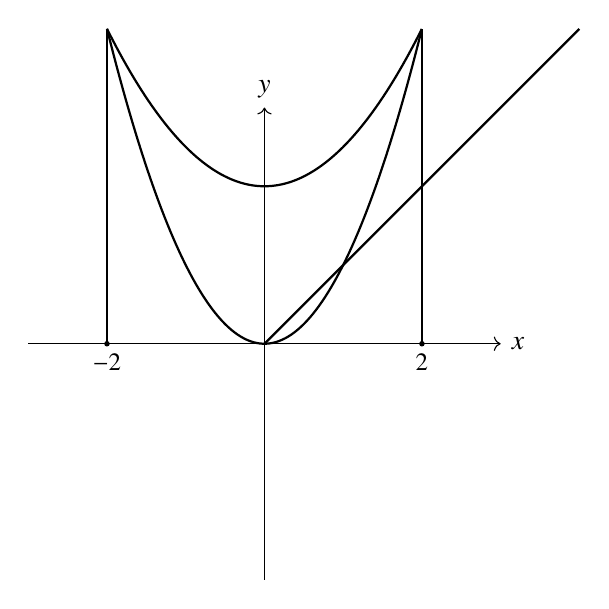
\begin{tikzpicture}
                \draw[black, thick, domain=-2:2, samples=100] 
                plot ({\x}, {((\x)^2}); 
                \draw[black, thick, domain=-2:2, samples=100] 
                plot ({\x}, {(0.5*(\x)^2 + 2});
                \draw[black, thick, domain=0:4, samples=100] 
                plot ({-2}, {((\x)});
                \draw[black, thick, domain=0:4, samples=100] 
                plot ({2}, {((\x)});
                \draw[black, thick, domain=0:4, samples=100] 
                plot ({\x}, {((\x)});
                \draw[->] (-3, 0) -- (3, 0) node[right] {$x$}; 
                \draw[->] (0, -3) -- (0, 3) node[above] {$y$};	
                \fill[black] (-2, 0) circle (1pt) node[below] {\small $-2$};
                \fill[black] (2, 0) circle (1pt) node[below] {\small $2$};
            \end{tikzpicture}
        \end{figure}
\end{enumerate}
\end{document}



